\documentclass{article} % For LaTeX2e
\usepackage{nips15submit_e,times}
\usepackage{hyperref}
\usepackage{url}
\usepackage{listings}
\usepackage{float}
\usepackage{amsmath,amsthm,amssymb,graphicx,mathtools,tikz}

\usepackage[noend]{algpseudocode}
\usepackage{algorithm}

\lstset{ %
	language = C, 
	language = C++,                		
	language=Matlab,
	language=Python,
	basicstyle=\ttfamily\footnotesize,        
	keywordstyle=\color{blue}\ttfamily,
	stringstyle=\color{red}\ttfamily,
	commentstyle=\color{magenta}\ttfamily,
	numberstyle = \footnotesize,      	
	numbers = left,                   		
	stepnumber = 1,                   	
	numbersep = 5pt,                  	
	backgroundcolor = \color{white},  	
	showspaces = false,               		
	showstringspaces = false,      		
	showtabs = false,                		
	frame = single,          			
	tabsize = 4,         				
	captionpos=b,          				
	breaklines=true,        			
	breakatwhitespace=false,    		
	escapeinside={\%*}{*)}     
}

\title{CSE 202: Algorithm Design and Analysis \\ Homework Assignment 1}

\author{
  Mingyang Wang, Ding Wang, Zhimin Zhou\\
  Department of Computer Science\\
  University of California, San Diego\\
  \texttt{\{miw092, diw005, zhz249\}@eng.ucsd.edu}\\
  A53100579 A53089251 A53089795\\
}

\newcommand{\fix}{\marginpar{FIX}}
\newcommand{\new}{\marginpar{NEW}}

\nipsfinalcopy % Uncomment for camera-ready version

\begin{document}

\maketitle
\section*{Problem 1}

\begin{enumerate}
\item
	
    True. Proof by example.
    
    First we say the $n$ \texttt{union} operations are formatted in the following way:
    
    at first each variable is in its separate set and after that every \texttt{union} is to union the roots of two subsets of variables next to each other. This means that There will be only one last set of variables after operations, and it will form a well-balanced binary tree. Then we conduct the \texttt{find} operations.
    
    Suppose all $m$ external \texttt{find} operations are called to find the root of the leaves of this well-balanced binary tree, then each \texttt{find} operation takes $\Omega(\mathtt{log}n)$ and in total the such a sequence takes $\Omega(m\mathtt{log}n)$.

\item
	
    Proof by contradiction. 
  
	Assume there is a MST $T$ and $e$ is not in it. Then we can add $e$ into $T$. This will lead to a cycle $C$ which contains $e$.

	We could always remove any other edge from cycle $C$ since every other edge in $c$ has a bigger weight than $e$. After that, we will still have a tree but this tree will have a smaller weight compared with $T$. Therefore $T$ is not a MST and we have found a contradiction.

\item

  	False. 
  
	We could have this cycle $C$ with 4 nodes. Each edge has weight bigger than 100. (Let's assume that the smallest weight edge in $C$ has a weight of 100). And between each 2 neighbor nodes in this cycle $C$, there is another path which contains one more node and forms a triangle cycle with these 2 nodes. Let's further assume that each edge in this triangle has a weight of 1. In this situation, the MST will have no edge from $C$.
    
    Below is the picture illustration, the center cycle is $C$:
    
    \begin{figure}[H]
    \centering
	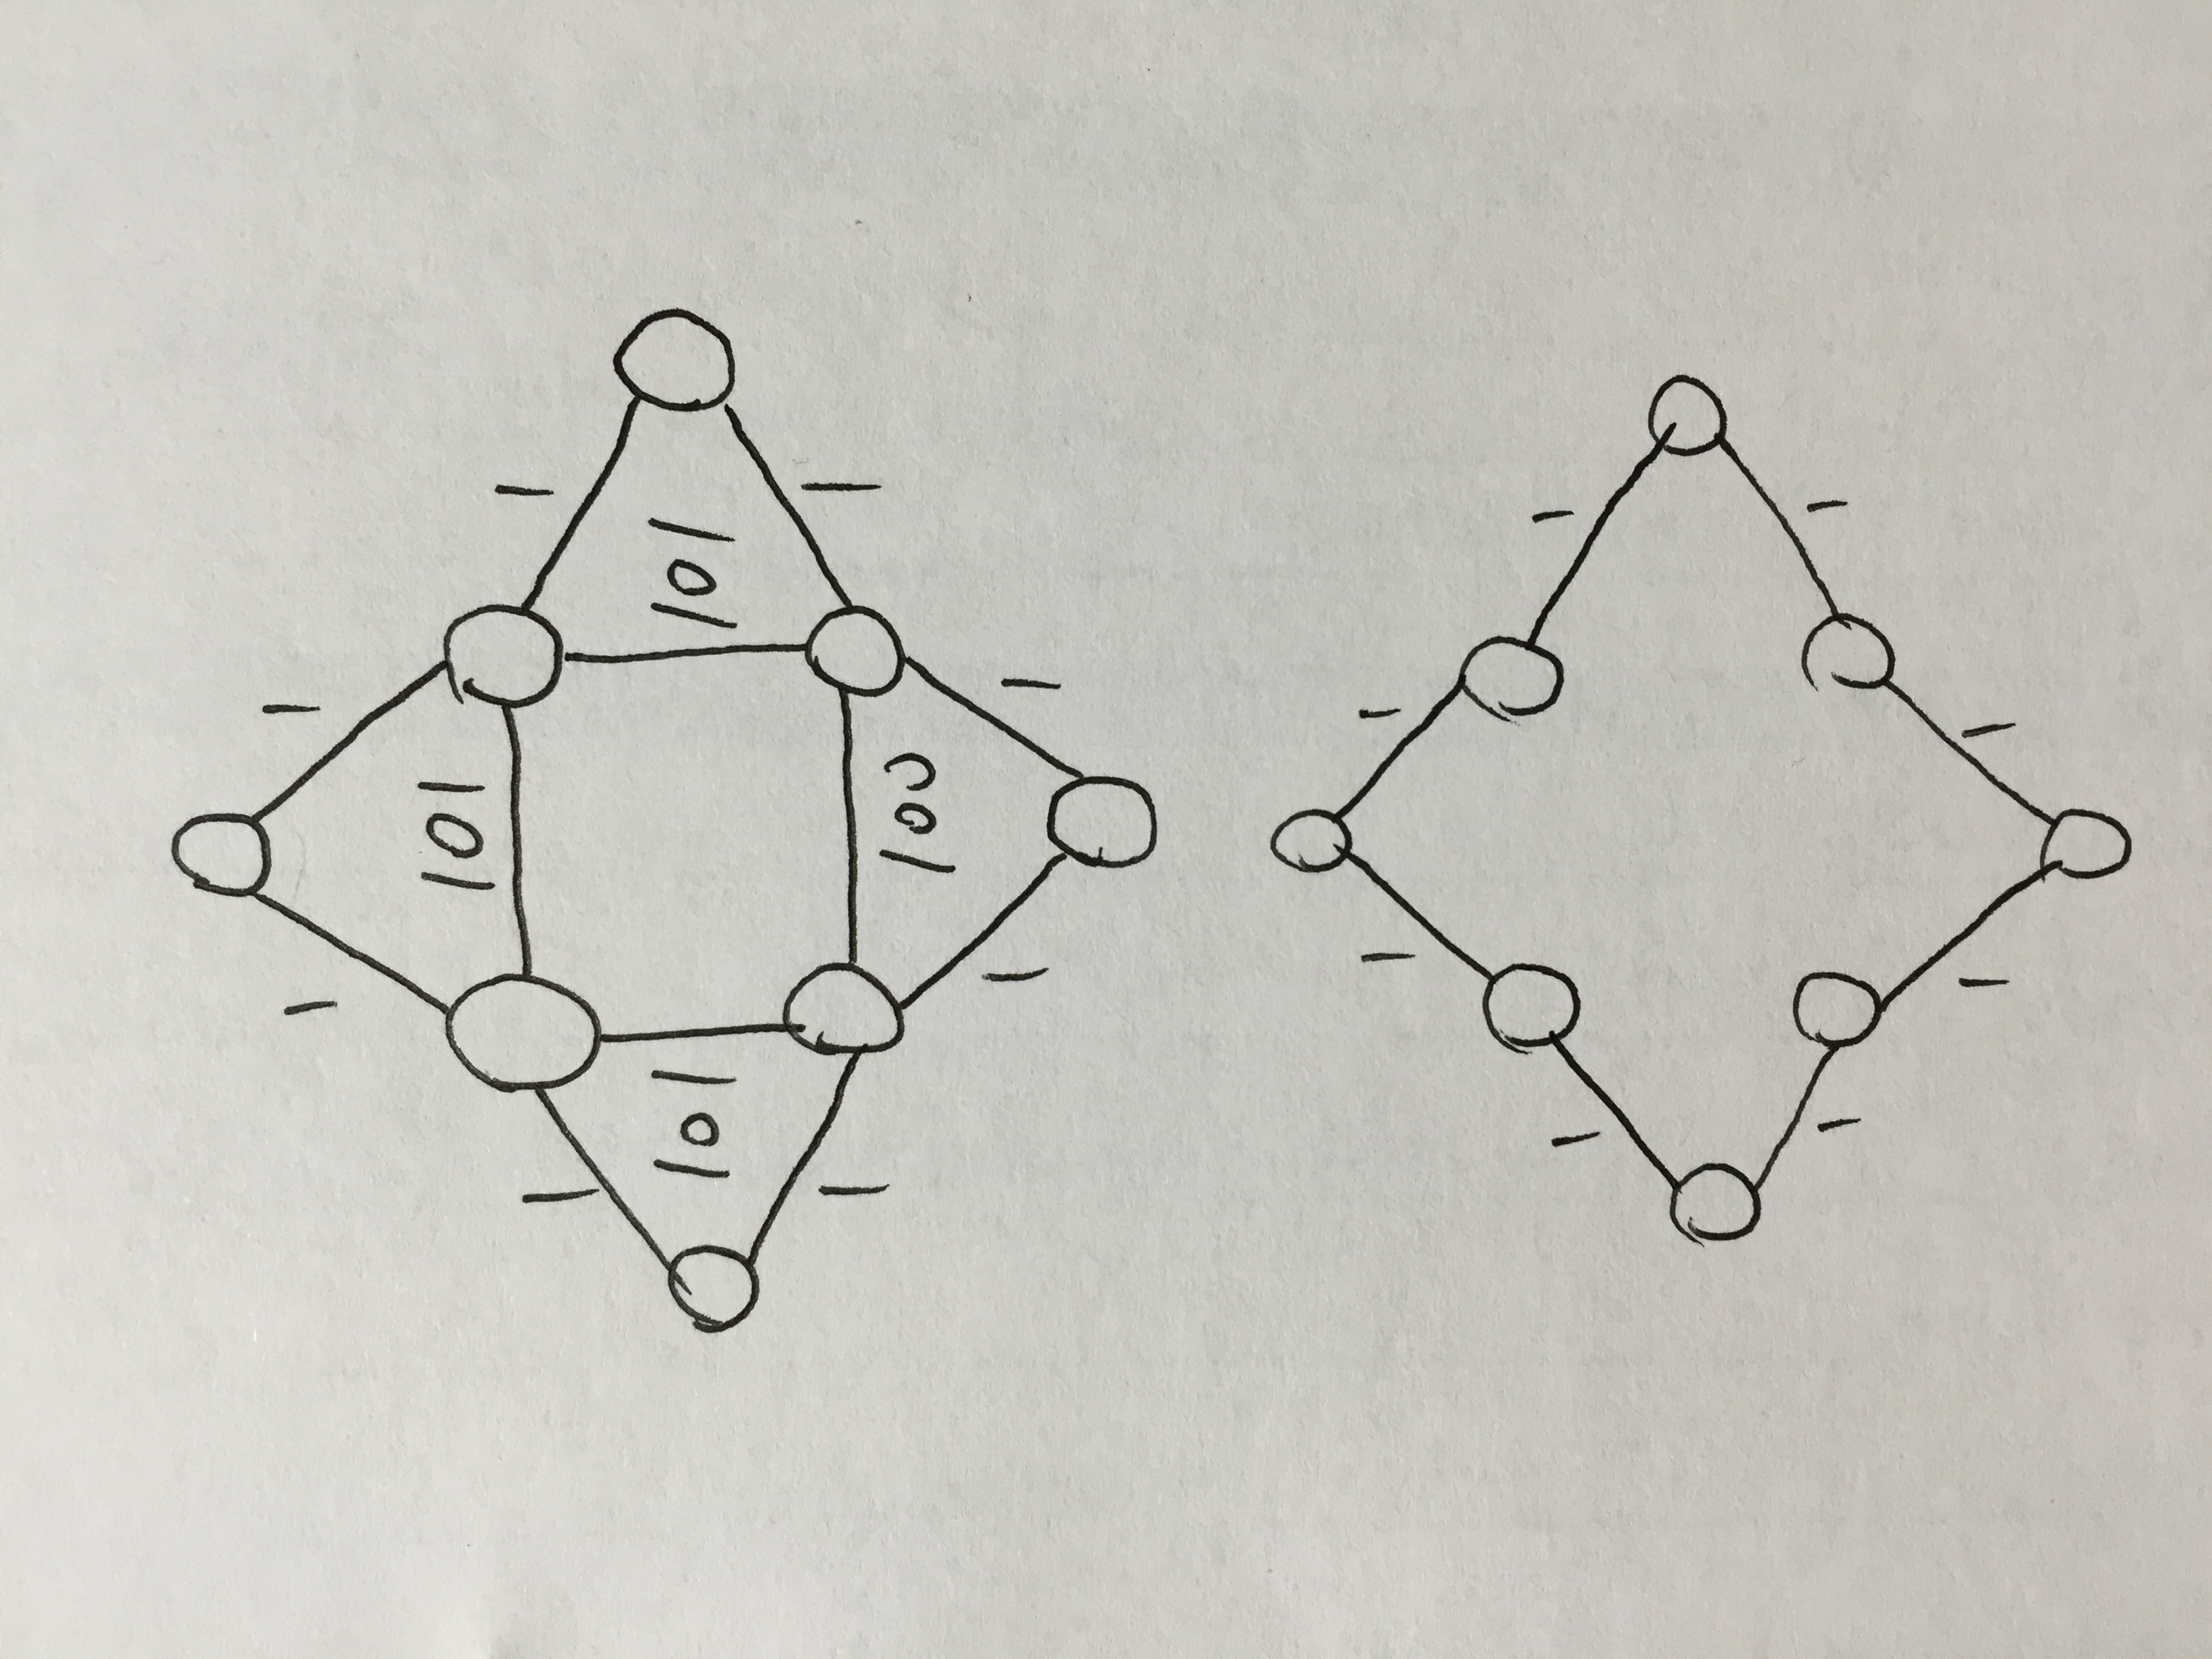
\includegraphics[width=\columnwidth, angle=270, scale=0.4]{pics/HW1_3.jpeg}
	\end{figure}

\item

  	Same as problem 3.

  	False. 
  
  	We could have this cycle $C$ with 4 nodes. Each edge has weight bigger than 100. And there is another path including one more node between each 2 nodes which only cause 2 more weight. In this situation, the MST will have no edge from $C$. Details can be seen in the above picture. The center cycle will never have any edge in any MST, thus false.

\item

  	Proof by contradiction.

	Assume $T_1$ and $T_2$ are two different MSTs. Lets say $e_1$ is the edge with smallest weight that is in $T_1$ but not in $T_2$.
    
    Then we add $e_1$ into $T_2$ and we get a cycle. Therefore one edge in the cycle we call it $e_2$ is not in $T_1$.

	We know that the weight of $e_2$ is bigger than the weight of $e_1$, and therefore we know $T_2$ = $T_1$ $\cup$ $\{e_2\}$ $\setminus$ $\{e_1\}$ has a total weight bigger than $T_1$. Therefore it is not a valid MST. Contradiction found.

\end{enumerate}

\newpage
\section*{Problem 2}
\begin{enumerate}
\item 1, 3, 3, 1
\item
	\begin{enumerate}
	\item 
    	Assume that $i \leq d_1 + 1, j > d_1 + 1$ and there is a link between $v_1$ and $v_j$. Then we can have $(v_1, v_i) \notin E \text{ and } (v_1, v_j) \in E$.

		Another thing is that we know that the degree of $v_i$ should be bigger than or equal to $v_j$, and since we already have $(v_1, v_i) \notin E \text{ and } (v_1, v_j) \in E$. We know that there must be another node $u$ that $(u, v_i) \in E \text{ and } (u, v_j) \notin E$.

	\item 
    	The changes need to be made could be from part(a). Namely we could first remove the edge $(v_1, v_j)$, then we pick any $v_i$ such that $2 \leq i \leq d_1+1$, and we add the edge $(v_1, v_i)$. Then we find a node $u$ of neighbor $v_i$ which is not a neighbor of $v_j$, and we remove the edge $(u, v_i)$ and replace with another edge $(u, v_j)$.
    
    	By doing this, we could have each node degree unchanged but generated the required edge $(v_1, v_i)$.

  	\item 
    	By combining prat(a) and part(b). We could know that for each neighbor of $v_1$ that is not belongs to $v_2 \text{ to } v_{d_1+1}$, we would have another $u \in V$ that $(u, v_i) \in E \text{ and } (u, v_j) \notin E$, $(v_1, v_i) \notin E \text{ and } (v_1, v_j) \in E$. Therefore according to part(b), we could always transform the above pair and get rid of edge $(u, v_j)$ and get a new edge $(u, v_i)$.

  	\end{enumerate}

\item 
	Algorithm
    \begin{algorithm}
    \caption{Check Graph Existence}
    \label{graphalgo}
    \begin{algorithmic}[1]
    \Function{Graph\textendash Exist($D$)} {}
    \State $n \gets \mathtt{size}(D)$

    \For{$d$ in $D$}
      \If {$d > n-1$} \Return false
      \EndIf
    \EndFor

    \If {$\mathtt{sum}(D)$ is not even} \Return false
    \EndIf

    \State Sort $D$ in descending order and record the mapping

    \For{$i$ in $(1,\dots,n-1)$}
      \If {$d_i < 0$} \Return false
      \EndIf
      \For{$j$ in $(1,\dots,d_i)$}
          \State Create edge $(i,i+j)$
          \State $d_{i+j} \gets d_{i+j} - 1$
      \EndFor
    \EndFor

	\If {$d_n \neq 0$} \Return false
	\EndIf

    \State \Return true
    \EndFunction
    \end{algorithmic}
	\end{algorithm}
    
    \begin{itemize}
	\item Proof of correctness: If there exists an degree that is larger than the limit ($n-1$) or the total degree is odd, such a graph must not exist. Then, based on the results in part 2, we conclude that the original problem is equivalent as finding such a degree sequence with descending order in which for any node,  all its connected nodes are its close neighbors. Hence, if we loop over all nodes, create corresponding edges between neighbors, and find out that some nodes' degrees are negative or the last node still has free degree at the end, such a graph must not exist as well.
    \item Time Complexity: Based on our algorithm, the running time is $O(2n + n\mathtt{log}n + 2m) = O(m+n\mathtt{log}n).$
	\end{itemize}

\end{enumerate}

\newpage
\section*{Problem 3}
\begin{enumerate}
\item
	We can treat each intersection as a node $v$ in a undirected connected graph $G(V,E)$. And each road as a edge $e$ between node in $G$. We can have a initialized set of all the edges $R$. Every time we pick up a node $v$ from the graph $G$, we can remove all the edges linked $v$ from $R$.
    
    \begin{itemize}
	\item Inputs: An undirected, connected graph $G(V,E)$ and the corresponding edge set $R$. This graph G should not contain self-loops (edges with both endpoints equal to the same node) or multiple edges between the same pair of nodes.
    \item Constraints: Pick up as few as possible nodes to make $R$ finally empty. Every time we pick up a node $v$ from the graph $G$, we can remove all the edges linked $v$ from $R$.
    \item Outputs: A set $S$ of nodes we picked up as well as the size of the $S$.
	\end{itemize}

\item
	False.
    
	The example is attached below:
    %Insert a graph here
    \begin{figure}[H]
    \centering
	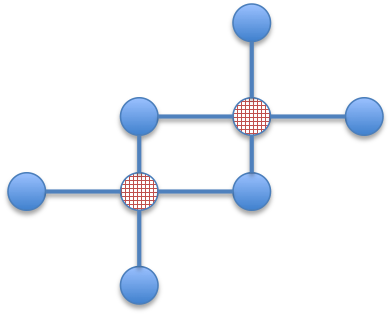
\includegraphics[width=\columnwidth, angle=0, scale=0.4]{pics/hw1_3_correct.png}
	\caption{optimal choices of intersections}
	\end{figure}
    
    \begin{figure}[H]
    \centering
	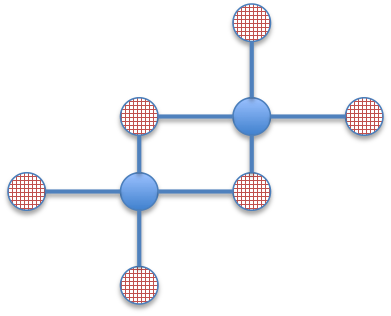
\includegraphics[width=\columnwidth, angle=0, scale=0.4]{pics/hw1_3_wrong.png}
	\caption{choices of intersections of this algorithm}
	\end{figure}
    
\item
	This algorithm does not works correctly either.
    
	The example is attached below:
    
    \begin{figure}[H]
    \centering
	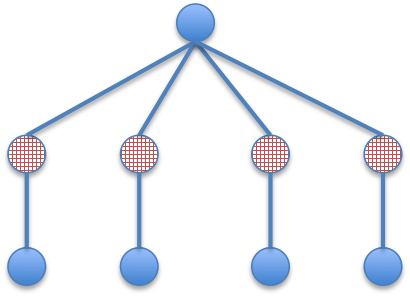
\includegraphics[width=\columnwidth, angle=0, scale=0.4]{pics/hw3_3_correct.png}
	\caption{optimal choices of intersections}
	\end{figure}
    
    \begin{figure}[H]
    \centering
	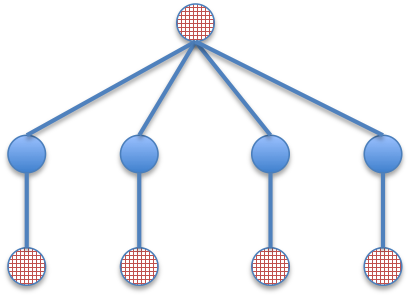
\includegraphics[width=\columnwidth, angle=0, scale=0.4]{pics/hw3_3_wrong.png}
	\caption{choices of intersections of this algorithm}
	\end{figure}

    
\end{enumerate}
\end{document}